
\chapter{Verification of integration}
\label{cha:integration}

Figure~\ref{fig:scope-of-code-verification} on Page~\pageref{fig:scope-of-code-verification}
outlines the scope of code verification within OpenETCS.
Verification activities, however, also concern integration of the \isoc~code
with the \scade model (see Section~\ref{sec:integration-with-model})
and with the communication layers that underlies the bit stream abstractions
(see Section~\ref{sec:integration-with-communication}).

\section{Integration with \scade model}
\label{sec:integration-with-model}

The generated data packets from Chapter~\ref{cha:packets}
are sent and received over the so-called \emph{bit stream} layer
(see Chapter~\ref{cha:bitstream}).
In order to exchange the packets with the OpenETCS application
layer that is modeled in \scade (see Figure~\ref{fig:scope-of-code-verification})
the so-called \emph{integer stream} layer was defined.
Due to the relative late emergence of this layer in the OpenETCS project
this layer could not be formally be verified.
Rather it was tested together with underlying communication layer
(see Section~\ref{sec:integration-with-communication}).


\section{Integration with the underlying communication layer}
\label{sec:integration-with-communication}

The ETCS packets and messages which are decoded represent the bit
decoding and encoding layer as applied inside the
BTM and EURORADIO module as described inside\footnote{%
	See SUBSET-026, Chapter 2, Figure 1.
}.

Concerning the ETCS air gap messages it represents the layer for
bit encoding and decoding the ETCS content  
\begin{itemize}
\item \inl{coded_EUROBALISE_input_telegram}
\item \inl{coded_EURORADIO_output_msg} and
\item \inl{coded_EURORADIO_input_msg}
\end{itemize}

between the openETCS Kernel and the OpenETCS API (see Figure~\ref{fig:integration}).


\begin{figure}[hbt]
\begin{center}
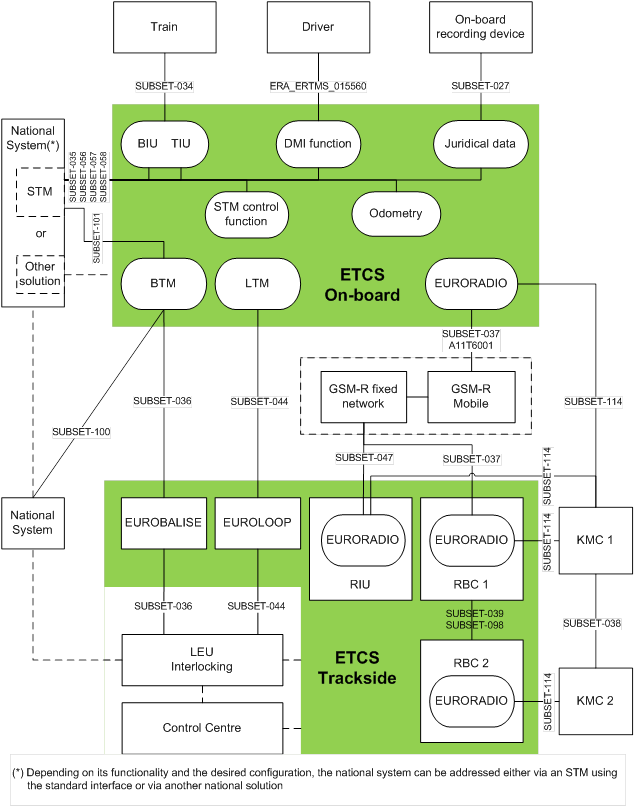
\includegraphics[width=0.99\textwidth]{figures/integration.png}
\caption{\label{fig:integration}
        Overview on integration interfaces.}
\end{center}
\end{figure}

%\FloatBarrier

The scope of the ETCS data packets is aligned with the openETCS show case
Amsterdam-Utrecht.
Thus not the complete set of packets can be decoded.
The supported packets are listed inside Section~\ref{sec:data-packets}.
 
The OpenETCS decoder/encoder is referenced
as ``additional code components developed by other means''.\footnote{
	See Chapter 3.5 of Deliverable~2.3.
}.
It is generated from the requirement document of Subset-026-6
and SUBSET-026-7 to a XML model.
This model was verified manually against the SUBSET-026. 
Although not having a certified code generator the verification
is artifacts were verified after generation.
